\documentclass[12pt]{article}
\usepackage{hyperref}
\usepackage{amsmath, amssymb, amsfonts}
\usepackage[margin=1.2cm]{geometry}
\usepackage{xcolor}
\usepackage{graphicx}
\usepackage{enumitem}
\parindent 0pt
\newcommand{\lb}{\\$\left|\rightarrow\right.$}
\newcommand{\enter}{\\\textcolor{white}{1}}
\ExplSyntaxOn
\NewDocumentCommand{\bo}{m}
 {
   \bold_commas:n { #1 }
 }
\cs_new:Npn \bold_commas:n #1
 {
   \seq_set_split:Nnn \l_tmpa_seq { , } { #1 }
   \seq_map_indexed_function:NN \l_tmpa_seq \__bold_commas_aux:nn
 }
\cs_new:Npn \__bold_commas_aux:nn #1 #2
 {
   \textbf{#2}
   \int_compare:nNnTF { #1 } < { \seq_count:N \l_tmpa_seq }
     { , }
     { }
 }
\ExplSyntaxOff

\title{RF and Microwave Engineering (EX752 / EX716)\\[0.4em]\large Detailed PYQ}
\author{}
\date{\today}

\begin{document}
\maketitle
\vspace{6cm}
\textbf{Notes}
\begin{itemize}[noitemsep]
  \item Questions from Tribhuvan University, IOE (2069--2082 BS), 24 papers.
  \item Regular exam = \bo{bold}, Back exam = regular font.
  \item BEX programme (EX752 / EG785) = normal font, BEI programme (EX716) = \texttt{this monospace style}.
  \item EX716 (BEI, IV/I) 7 papers 2079--2082; EX752 (BEX, IV/II) 16 papers 2070--2080; EG785EX (BEX Elective II) 1 paper, 2069 Bhadra.
  \item A header printing ``Regular / Back'' in one box counts as Regular, so \bo{76 Bh} and \bo{71 Bh} are bold.
  \item So: \bo{72 Ash} = BEX Regular, 73 Ma = BEX Back, \bo{\texttt{79 Bh}} = BEI Regular, \texttt{81 Ba} = BEI Back.
  \item Months: Ba = Baishakh, Bh = Bhadra, Ash = Ashwin, Ma = Magh, Ch = Chaitra.
  \item Keywords: (I) = Importance/Need/Significance, (+) = Advantage, (-) = Disadvantage, +Fig = Figure, +Eg = Example, Vs = Compare/Differentiate.
\end{itemize}
\pagebreak
\tableofcontents
\pagebreak

%=======================================================================
\section{Introduction}
\begin{center}(3 Hours)\end{center}

  \subsection{Standard Frequency Bands \& Microwave Applications}
    \begin{enumerate}[topsep=0pt, noitemsep]
      \item Classify microwave frequency bands + major applications \hfill [4] (69 Bh)
        \lb How is the microwave frequency band classified by IEEE? \hfill [2+4] (\texttt{80 Ba})
        \lb Classify microwave frequency band + application in major areas \hfill [3+3] (\bo{\texttt{79 Bh}})
        \lb How is microwave frequency band classified by the IEEE? (+) (-) of microwaves compared to lower frequencies \hfill [5+5] (\bo{76 Bh})
      \item List areas of application of microwave systems \hfill [4] (\bo{70 Bh, 70 Ma})
        \lb List uses of microwaves in communication systems + detailed protocols of any three \hfill [2+6] (\texttt{81 Ba})
        \lb Areas of application + detailed protocols of two microwave communication systems \hfill [3+3+4] (\bo{\texttt{80 Bh}})
        \lb Real-world protocols of any three major applications of microwave communication systems \hfill [4+6] (\bo{\texttt{82 Bh}})
        \lb Specifications/protocols of any five microwave communication systems \hfill [4+4] (\texttt{82 Ba})
        \lb Lists the areas of application of microwave system (with operational-principle comparison) \hfill [10] (\bo{78 Ch})
    \end{enumerate}

  \subsection{Behaviour: Conventional Vs RF/Microwave Circuits}
    \begin{enumerate}[topsep=0pt, noitemsep]
      \item Lumped Vs distributed circuit analysis; uses of microwave bands \hfill [4+2] (73 Ma)
        \lb Differentiate lumped and distributed circuit analysis (+ protocols of two M/W comm systems) \hfill [3+3+4] (\bo{\texttt{80 Bh}})
      \item Microwave Vs conventional low-freq systems: working principles \hfill [4] (\bo{70 Bh, 70 Ma})
        \lb Compare behaviour of circuits for low-freq/conventional Vs RF/microwave bands \hfill [3+3] (\bo{\texttt{79 Bh}})
        \lb (+) (-) of microwaves over acoustic waves \hfill [5] (\bo{72 Ash})
        \lb (+) (-): microwave Vs conventional low-freq \hfill [6] (71 Ma)
        \lb (+) (-) of microwaves compared to lower frequencies \hfill [2+4] (\texttt{80 Ba})
        \lb Circuit at seismic band Vs RF/Microwave counterparts \hfill [8] (\bo{75 Bh})
        \lb Behavior of microwave passive components at low frequency bands Vs microwave bands \hfill [4+6] (\bo{\texttt{82 Bh}})
        \lb Unique differences between microwave and conventional low frequency systems \hfill [4+4] (\texttt{82 Ba})
        \lb Distinguish microwave and traditional low frequency systems by operating principle; why S-parameter based analysis is a must \hfill [5+3] (\bo{\texttt{81 Bh}})
        \lb How microwave systems are different from conventional low frequency devices \hfill [8] (\bo{80 Ch})
        \lb Based on operational principles, compare microwave systems with conventional low frequency systems \hfill [10] (\bo{78 Ch})
        \lb Behavior of microwave circuits; (+) (-) of using microwave frequency \hfill [4+4] (\bo{77 Ch})
        \lb Merits and demerits of microwaves compared to seismic wave \hfill [5] (72 Ma)
    \end{enumerate}

\pagebreak
%=======================================================================
\section{RF and M/W Transmission Lines}
\begin{center}(6 Hours)\end{center}

  \subsection{Types of Transmission Lines}
    \begin{enumerate}[topsep=0pt, noitemsep]
      \item Microwave transmission lines Vs conventional low-freq lines \hfill [4] (69 Bh)
      \item Microstrip Vs strip-lines \hfill [5] (71 Ma)
      \item Differentiate the behavior of a transmission line at conventional low frequency and microwave bands \hfill [10] (\bo{79 Ch})
    \end{enumerate}

  \subsection{Smith Chart / Admittance (Immittance) Chart}
    \begin{enumerate}[topsep=0pt, noitemsep]
      \item Admittance chart \hfill [2] (\bo{72 Ash})
      \item Immittance chart: sketch + list duality parameters \hfill [10] (\bo{75 Bh})
        \lb Sketch of an Immittance Chart (short note) \hfill [4] (\texttt{81 Ba})
        \lb Sketch an immittance chart and compare the scales \hfill [5] (72 Ma)
        \lb Immittance Chart (short note) \hfill [5] (\bo{80 Ch})
      \item Lossless $50\,\Omega$ line terminated by $75{+}j100\,\Omega$; using Smith Chart find (a) $\Gamma_L$, (b) VSWR, (c) $Z_{in}$ at $0.375\lambda$ from the load, (d) shortest length of line for which impedance is purely resistive, (e) the value of that resistance \hfill [10] (\bo{79 Ch})
    \end{enumerate}

  \subsection{Impedance Matching: Single Stub}
    \begin{enumerate}[topsep=0pt, noitemsep]
      \item Single stub shunt tuning (short \& open): $Z_L = 80{+}j100\,\Omega$, microstrip \hfill [2+8] (\bo{72 Ash})
      \item Single short/open shunt stub: $\Gamma_L = 0.5\angle51^\circ$, $Z_0 = 50\,\Omega$ +Smith Chart \hfill [8] (\bo{74 Bh})
      \item Single matching stub: $100\,\Omega$ lossless line, complex load $120{-}j160\,\Omega$; all design steps with reasoning; S-Matrix before and after \hfill [5+3+2] (\bo{\texttt{81 Bh}})
      \item Single short-circuited matching stub with self-defined line and load impedances, mentioning the steps \hfill [10] (\bo{79 Ch})
      \item Single-stub tuner matching a lossless line to an antenna load, any assumed placement and length; derive its S-matrix \hfill [10] (\bo{76 Bh})
      \item Signal shunt and open matching networks using Smith Chart: $Z_0 = 75\,\Omega$, $Z_L = 78.27{+}j60.93\,\Omega$; sketch the physical diagram considering microstrips \hfill [4+4+2] (72 Ma)
    \end{enumerate}

  \subsection{Impedance Matching: Double Stub}
    \begin{enumerate}[topsep=0pt, noitemsep]
      \item Double stub ($3\lambda/8$): $Z_L = 300{+}j300\,\Omega$, $Z_0 = 300\,\Omega$ +Fig \hfill [10] (71 Bh)
      \item Double stub ($3\lambda/8$): $Z_L = 80{+}j180\,\Omega$, $Z_0 = 100\,\Omega$, 3 GHz +Fig \hfill [10] (\bo{70 Bh})
      \item Double stub ($3\lambda/8$): $Z_L = 190{+}j110\,\Omega$, $Z_0 = 100\,\Omega$, 10 GHz +Fig \hfill [10] (70 Ma)
      \item Double stub: inductive load, $Z_0 = 50\,\Omega$ +Fig \hfill [8] (73 Ma)
      \item Double stub (short-circuit): $Z_L = 75{+}j75\,\Omega$, $Z_0 = 50\,\Omega$, $3\lambda/8$ \hfill [3+15] (69 Bh)
      \item Double stub (short-circuit): complex inductive load, $Z_0 = 78.0\,\Omega$ +Fig \hfill [8+2] (\bo{73 Bh})
      \item Double stub (short-circuit): $Z_L = 0.4{+}j0.85$ (normalized), $Z_0 = 75\,\Omega$ coaxial \hfill [10+2] (\bo{75 Bh})
      \item Double stub shunt tuner (open stubs, $3\lambda/8$, first at $0.4\lambda$): $Z_L = 60{-}j80\,\Omega$, $50\,\Omega$ line; prepare S-matrix \hfill [8+2] (\texttt{80 Ba})
      \item Double stub (short-circuited coaxial): $Z_L = 109{+}j120\,\Omega$, $75\,\Omega$ coaxial line; prepare S-matrix \hfill [8+2] (\bo{\texttt{80 Bh}})
      \item Double stub: $\Gamma_L = 0.64\angle58^\circ$, $Z_0 = 100\,\Omega$; prepare S-matrix of matched network \hfill [8+2] (\texttt{81 Ba})
      \item Double stub shunt tuner ($3\lambda/8$, first stub $0.01\lambda$ from load): $50\,\Omega$ lossless line, load admittance $0.00813{+}j0.0065\,\mho$ +Smith Chart; write S-parameter \hfill [8+2] (\bo{\texttt{79 Bh}})
      \item Broadband microstrip antenna, load reflection coefficient $0.33\angle66^\circ$, transmission patch $75\,\Omega$; design the matching stubs and express the scattering matrix of the matched network \hfill [10] (\bo{\texttt{82 Bh}})
      \item Double stub for an antenna at 10 GHz: $\Gamma = |0.45|\angle60^\circ$, $100\,\Omega$ line; sketch physical diagram using micro strips; S-Matrices before and after \hfill [10+2+2] (\texttt{82 Ba})
      \item Double stub ($3\lambda/8$): $Z_L = 110{+}j110\,\Omega$, $Z_0 = 100\,\Omega$; find lengths and spacing \hfill [12] (\bo{80 Ch})
      \item Different impedance matching techniques; resulting S-matrix of a perfectly matched double-stub network \hfill [4+6] (\bo{78 Ch})
      \item Sketch a double-stub perfectly matched network using microstrip and prepare its s-matrix \hfill [2+8] (\bo{77 Ch})
      \item (+) of double stub matching over single stub matching; steps for impedance matching of a load using a double-stub network +Eg, using the provided Smith Chart \hfill [2+8] (74 Ma)
    \end{enumerate}

\pagebreak
%=======================================================================
\section{RF and M/W Network Theory and Analysis}
\begin{center}(4 Hours)\end{center}

  \subsection{S-parameters: (I), Definition, Properties}
    \begin{enumerate}[topsep=0pt, noitemsep]
      \item S-parameters (I) in microwave network analysis \hfill [4] (\bo{70 Bh}, 69 Bh)
        \lb S-parameters (I); Vs h-parameters for network analysis \hfill [4+4] (70 Ma)
        \lb S-parameters (I) \hfill [4] (\bo{75 Bh})
      \item S-parameters for two-port network \hfill [4+5] (\bo{70 Bh})
        \lb S-parameters for two-port network \hfill [4+6] (69 Bh)
        \lb S-parameters for two-port network \hfill [4] (70 Ma)
        \lb Why are S-parameters used in microwave network analysis? Derive S-parameters for a two-port network \hfill [2+6] (\texttt{80 Ba})
        \lb Need of S-parameter + properties; three-port network parameters using E-plane Tee example \hfill [4+4] (\bo{\texttt{80 Bh}})
        \lb Compare h-parameters with S-parameter; describe S-parameters using a two-port network \hfill [5+5] (\bo{80 Ch})
        \lb Importance of S-parameters for microwave frequencies; evaluate the S-matrix of an Amplitude Modulator \hfill [3+7] (\bo{78 Ch})
      \item S-parameters for three-port network \hfill [5+2] (\bo{72 Ash})
        \lb S-matrix for 3-port network with +Eg \hfill [4+4] (73 Ma)
        \lb Properties of 3-port network \hfill [4+4] (\bo{73 Bh})
        \lb Three-port network model + its characteristic parameters \hfill [4] (\bo{\texttt{82 Bh}})
        \lb Analyze a three port network using S-parameters \hfill [2+6] (74 Ma)
      \item Return loss \& insertion loss \hfill [2] (\bo{72 Ash})
      \item Why are S-parameters used at high frequencies? For $[S]=\begin{bmatrix}0.4{+}j0.5 & j0.6\\ j0.6 & 0.4{-}j0.5\end{bmatrix}$: (a) reciprocal? (b) lossless? (c) return loss at input? (d) if input power is 5 W, reflected power? \hfill [3+1+1+1+2] (\bo{\texttt{79 Bh}})
    \end{enumerate}

  \subsection{Passive Microwave Devices: S-matrix Analysis}
    \begin{enumerate}[topsep=0pt, noitemsep]
      \item Identify + explain passive device from S-matrix (4-port) \hfill [8] (\bo{74 Bh})
      \item Passive device from given S-matrix: judge condition + characteristics \hfill [6] (\bo{75 Bh})
      \item Choose device to split power in half + explain properties \hfill [8] (73 Ma)
        \lb Two radar transmitters, double power to antenna: solution +Fig, math \hfill [8] (\bo{73 Bh})
      \item Prepare S-Matrices of a perfectly working E-Plane Tee, H-Plane Tee and a Duplexer, and explore their uses \hfill [8] (\texttt{81 Ba})
      \item Find the basic differences of the systems having the S-Matrix sets (a) $S_{11}{=}0.65\angle146^\circ$, $S_{12}{=}0.12\angle46^\circ$, $S_{21}{=}2.30\angle44^\circ$, $S_{22}{=}0.17\angle{-172^\circ}$ and (b) $S_{11}{=}0.30\angle{-134^\circ}$, $S_{12}{=}0.03\angle46^\circ$, $S_{21}{=}2.20\angle44^\circ$, $S_{22}{=}0.10\angle{-172^\circ}$ \hfill [4] (\bo{\texttt{82 Bh}})
      \item Identify and explain, with a neat diagram, the passive device described by the 4-port S-Matrix $\begin{bmatrix}S_{11}&S_{12}&S_{13}&S_{14}\\ S_{12}&S_{22}&S_{13}&-S_{14}\\ S_{13}&S_{13}&0&0\\ S_{14}&-S_{14}&0&0\end{bmatrix}$ \hfill [5] (\bo{\texttt{81 Bh}})
      \item Identify and explain the properties of the passive device with S-Matrix $\begin{bmatrix}0&0&1&1\\ 0&0&-1&1\\ 1&-1&0&0\\ 1&1&0&0\end{bmatrix}$ +Fig \hfill [10] (\bo{78 Ch})
      \item Airport Surveillance Radar requiring half the input power to the antenna than the transmitter can deliver, using a duplexer; prepare its S-matrix \hfill [10] (\bo{76 Bh})
      \item Two identical radar transmitters, twice the input power to an antenna; give the solution with explanation using S-matrix \hfill [6] (74 Ma)
    \end{enumerate}

\pagebreak
%=======================================================================
\section{RF/Microwave Components and Devices}
\begin{center}(8 Hours)\end{center}

  \subsection{Waveguides}
    \begin{enumerate}[topsep=0pt, noitemsep]
      \item Rectangular waveguide: TE mode field equations \hfill [7+3] (\bo{70 Bh})
        \lb Rectangular waveguide: TM mode field equations + parameters \hfill [8+2] (71 Bh)
        \lb Rectangular waveguide: TM mode field equations \hfill [7+3] (70 Ma) [10] (\bo{74 Bh})
        \lb Rectangular waveguide: modes of propagation + critical parameters \hfill [8] (69 Bh)
        \lb Field equations + basic characteristic equations of rectangular waveguide, $\text{TM}_{11}$ mode \hfill [8] (\texttt{81 Ba})
        \lb $\text{TE}_{mn}$ field equations of rectangular waveguide (short note) \hfill [4] (\bo{\texttt{80 Bh}})
        \lb Express various field components of a rectangular waveguide in TM mode \hfill [8] (\bo{\texttt{81 Bh}})
        \lb EM field equations and characteristic parameters of a rectangular waveguide working on TE mode \hfill [10] (\bo{80 Ch})
        \lb Basic field equations of a rectangular waveguide working at TE mode \hfill [10] (\bo{79 Ch})
        \lb Derive explicitly the field equations of rectangular waveguides for TE modes \hfill [8] (\bo{77 Ch})
        \lb Field and characteristics equations of a rectangular wave guide working in TM mode \hfill [10] (\bo{76 Bh})
        \lb Field equation of rectangular wave guide for TE mode (short note) \hfill [4] (74 Ma)
        \lb TM mode rectangular wave guide (short note) \hfill [5] (72 Ma)
      \item $\text{TE}_{10}$ Vs $\text{TE}_{20}$: cutoff frequency + dominant mode \hfill [2] (71 Bh)
        \lb Show 1 GHz cannot propagate in $\text{TE}_{10}$, 5 cm wall separation \hfill [3] (\bo{70 Bh})
        \lb Prove $\text{TM}_{01}$ and $\text{TM}_{10}$ modes do not exist \hfill [3] (70 Ma)
        \lb Prove that the lowest cut-off frequency mode in rectangular waveguides operating in TM mode is $\text{TM}_{11}$ \hfill [3] (\bo{\texttt{82 Bh}})
        \lb Show that the dominant mode in rectangular waveguides operating in TE mode is $\text{TE}_{10}$ when $b>a$ \hfill [3] (\bo{\texttt{81 Bh}})
        \lb Degenerative and dominant modes of a rectangular waveguide +Eg \hfill [3] (\texttt{82 Ba})
        \lb Dominant Vs degenerate modes; for $a = 3b$ find the dominant mode among $\text{TM}_{01}$, $\text{TM}_{10}$, $\text{TM}_{11}$, $\text{TM}_{21}$, $\text{TM}_{12}$, $\text{TM}_{02}$, $\text{TM}_{20}$ \hfill [2+2] (72 Ma)
      \item TE Vs TM mode: circular waveguide \hfill [10] (71 Ma)
        \lb Fundamental field + characteristic equations of a circular waveguide, TE mode \hfill [10] (\bo{\texttt{79 Bh}})
        \lb Electromagnetic field equations of a circular waveguide operating at TE Mode \hfill [7] (\texttt{82 Ba})
      \item Circular waveguide: TM wave field strength + dominant mode (TE \& TM) \hfill [8+2] (\bo{75 Bh})
      \item Dominant mode in waveguide \hfill [5] (\bo{72 Ash})
        \lb What is dominant mode? Dominant modes for rectangular \& circular waveguides. Does a rectangular waveguide of width 2.254 cm support 6 GHz? \hfill [1+1+2] (\bo{\texttt{80 Bh}})
      \item For an air-filled rectangular waveguide (width 3 cm, $f=6$ GHz, dominant mode): find cutoff frequency, cutoff wavelength, group velocity, phase velocity, guide wavelength and characteristic impedance. Also explain the four basic parameters of a directional coupler. \hfill [6+4] (\texttt{80 Ba})
      \item Rectangular waveguide with suitably assumed breadth, width and frequency (dominant mode): determine cut-off frequency, phase velocity, propagation wavelength in the waveguide and the characteristic impedance \hfill [6] (\bo{77 Ch})
    \end{enumerate}

  \subsection{Coupling: Probes and Loops}
    \begin{enumerate}[topsep=0pt, noitemsep]
      \item PROBE-coupling Vs LOOP-coupling \hfill [5] (69 Bh)
    \end{enumerate}

  \subsection{Tee Junctions}
    \begin{enumerate}[topsep=0pt, noitemsep]
      \item Waveguide junctions; Magic Tee operational principles (S-parameters) \hfill [3+3] (\bo{72 Ash})
        \lb Microwave magic tee \hfill [5] (71 Ma, 71 Bh)
        \lb Draw a neat diagram of a magic tee and derive its S-parameter \hfill [4] (\bo{\texttt{80 Bh}})
        \lb Microwave Magic Tee (short note) \hfill [4] (\bo{\texttt{79 Bh}})
        \lb S-Matrix of a rectangular magic tee having both E and H-arms shorted, and how it behaves \hfill [4] (\bo{\texttt{82 Bh}})
        \lb Microwave magic tee (short note) \hfill [5] (\bo{80 Ch})
        \lb Magic Tee (short note) \hfill [5] (\bo{79 Ch})
        \lb Describe magic Tee based on S-parameters \hfill [6] (72 Ma)
      \item E-plane tee Vs H-plane tee \hfill [5] (69 Bh)
        \lb E-plane Tee (short note) \hfill [4] (\texttt{80 Ba})
      \item Hybrid tee \hfill [8] (70 Ma)
      \item Properties of a Hybrid-Tee, using proper S-Matrices, for (a) terminated E-arm, (b) terminated H-arm and (c) terminated co-planner arms \hfill [4+4+2] (\texttt{82 Ba})
      \item Properties of two Magic Tees with their E-arms connected; derive its S-matrix \hfill [10] (\bo{77 Ch})
      \item Combitional effect of two magic fees connected in H-plane (short note) \hfill [5] (\bo{78 Ch})
      \item 3-port directional coupler (S-parameters analysis) \hfill [4] (\bo{75 Bh})
    \end{enumerate}

  \subsection{Directional Couplers}
    \begin{enumerate}[topsep=0pt, noitemsep]
      \item Directional couplers \hfill [6] (73 Bh)
      \item Directional coupler (short note) \hfill [5] (\bo{79 Ch})
    \end{enumerate}

  \subsection{Other Devices (Gunn diode, MASER)}
    \begin{enumerate}[topsep=0pt, noitemsep]
      \item Gunn-diode (short note) \hfill [4] (\bo{\texttt{79 Bh}})
      \item MASER (short note) \hfill [4] (\texttt{80 Ba})
    \end{enumerate}

  \subsection{Resonators and Circulators}
    \begin{enumerate}[topsep=0pt, noitemsep]
      \item Circulators \hfill [5] (\bo{72 Ash}, 70 Bh, 73 Ma)
      \item Microwave cavity resonators \hfill [6] (\bo{74 Bh})
      \item Cavity Resonators (short note) \hfill [4] (74 Ma)
    \end{enumerate}

  \subsection{Microstrips}
    \begin{enumerate}[topsep=0pt, noitemsep]
      \item Microstrips \hfill [5] (69 Bh)
    \end{enumerate}

\pagebreak
%=======================================================================
\section{Microwave Generators}
\begin{center}(5 Hours)\end{center}

  \subsection{Transit-time Effect}
    \begin{enumerate}[topsep=0pt, noitemsep]
      \item Transit-time effect + two-cavity klystron construction \& operation \hfill [2+8] (70 Ma)
      \item What is transit time effect? Working principles of a magtron having $45^\circ$ phase difference of adjacent cavities \hfill [2+6] (\bo{77 Ch})
    \end{enumerate}

  \subsection{Klystrons}
    \begin{enumerate}[topsep=0pt, noitemsep]
      \item Bunching effect (density modulation) \hfill [2] (\bo{72 Ash}, 71 Bh, 70 Bh, 70 Ma)
      \item Bunching effect and field effect; working principle of a microwave high power oscillator employing both +Fig \hfill [2+2+4] (\bo{\texttt{81 Bh}})
      \item Multi-cavity klystron oscillator working principle \hfill [2+7] (\bo{72 Ash}) [2+8] (71 Bh)
        \lb Two-cavity klystron \hfill [5] (69 Bh)
        \lb Multi-cavity Klystron Amplifier (short note) \hfill [4] (\texttt{82 Ba})
        \lb Multi-cavity klystron (short note) \hfill [5] (\bo{80 Ch})
        \lb Cross-field effect; construction and principle of operation of a multi cavity klystron amplifier \hfill [2+8] (\bo{78 Ch})
        \lb Bunching effect in reflex klystron (short note) \hfill [5] (72 Ma)
      \item Velocity modulation + bunching in multicavity reflex klystron +Fig \hfill [10] (\bo{75 Bh})
    \end{enumerate}

  \subsection{TWT and Magnetrons}
    \begin{enumerate}[topsep=0pt, noitemsep]
      \item Cavity magnetron: construction + operational features \hfill [2+8] (\bo{70 Bh}) [10] (71 Ma)
        \lb Sketch a cross-sectional magnetron with $45^\circ$ phase shift among adjacent cavities; explain its functioning as a power amplifier + bunching effect \hfill [6+2] (\texttt{80 Ba})
        \lb Working principles of a cross-field magnetron with $60^\circ$ phase differences among adjacent cavities \hfill [8] (\texttt{81 Ba})
        \lb Working principle of a circular beam-type microwave cavity-controlled cross-field amplifier \hfill [7] (\bo{\texttt{82 Bh}})
        \lb Magnetron (short note) \hfill [5] (\bo{79 Ch})
        \lb Working principle and applications of a cavity magnetron having $45^\circ$ phase shift between the cavities \hfill [8] (74 Ma)
        \lb Cross-field effect; design and working principle of a cross field cavity device for power amplifier, $90^\circ$ phase shift between adjacent cavities \hfill [3+7] (72 Ma)
      \item What is bunching effect? Describe the construction and operation of Traveling Wave Tube (TWT) \hfill [2+6] (\bo{\texttt{80 Bh}})
        \lb How is the output of conventional tubes reduced at microwaves (inter-electrode capacitance, lead inductance, transit time)? Construction \& working of TWT \hfill [2+6] (\bo{\texttt{79 Bh}})
    \end{enumerate}

  \subsection{Backward Wave Oscillator (BWO) and LNA}
    \begin{enumerate}[topsep=0pt, noitemsep]
      \item BWO: slow backward wave structure, construction + principle \hfill [2+8] (73 Ma) [5] (\bo{74 Bh})
      \item LNA: construction + working principle \hfill [2+6] (73 Bh)
    \end{enumerate}

\pagebreak
%=======================================================================
\section{RF Design Practices}
\begin{center}(10 Hours)\end{center}

  \subsection{RF Filter: Insertion Loss Method \& Microstrip Implementation}
    \begin{enumerate}[topsep=0pt, noitemsep]
      \item LNA cavity device -- insertion loss method for filter design \hfill [5] (\bo{72 Ash})
      \item Insertion loss method for filter design \hfill [5] (\bo{75 Bh}) [8] (73 Bh)
        \lb Butterworth \& Chebyshev: common to two-port prototype filter (insertion loss) \hfill [4] (\bo{70 Bh}, 70 Ma)
        \lb Describe insertion loss method, illustrate passive LPF using $\mu$-strip \hfill [8+2] (73 Ma)
      \item Microwave filter design procedures \hfill [5] (71 Bh)
        \lb Designing steps + passive HPF +Eg using microstrips \hfill [6+4] (\bo{74 Bh})
        \lb Steps of microwave filter designing; sketch a double-pad T-type passive filter using microstrip \hfill [7+3] (\texttt{81 Ba})
        \lb Why filters are designed using the Insertion Loss Method; detail design steps of the filter below, implemented using microstrip \hfill [3+8+3] (\bo{\texttt{82 Bh}})
        \\ \mbox{}\hfill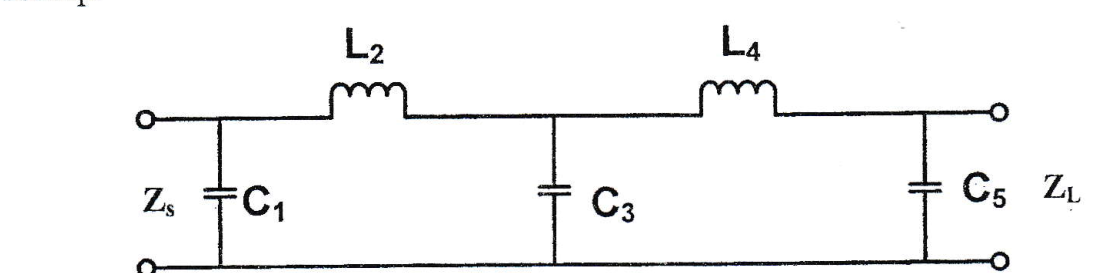
\includegraphics[width=4.6in]{images/rf_82bh_filter.png}\hfill\mbox{}
        \lb Microwave filter designing steps; sketch of a triple-pad series-arm type HPF using micro strips \hfill [7+3] (\texttt{82 Ba})
        \lb Single section series arm passive BPF +Eg using microstrip; how filters are designed using the Insertion Loss Method \hfill [2+8] (\bo{\texttt{81 Bh}})
        \lb Double-section series-arm type micro strip filter designed using insertion loss method \hfill [10] (\bo{78 Ch})
        \lb Procedures for prototyping Butterworth LPF using insertion loss method \hfill [8] (\bo{77 Ch})
        \lb LPF prototype (Butterworth \& Chebyshev) via insertion loss; implement a LPF double $\pi$-sections using microstips \hfill [8+2] (\bo{76 Bh})
        \lb How is a LPF implemented using microstrip? How are LPFs prototyped? \hfill [5+3] (74 Ma)
        \lb Microwave filter parameters and LPF prototyping (short note) \hfill [5] (72 Ma)
      \item LPF using microstrip + how prototyped \hfill [3+5] (\bo{72 Ash})
        \lb Why is the insertion loss technique used to design microwave filters? Sketch a double-section shunt-arm microwave LPF using microstrips \hfill [3+5] (\texttt{80 Ba})
        \lb How is a LPF prototyped based on Butterworth/Chebyshev and converted to other filters? Implement a 2nd-order HPF $\pi$-section using microstrips \hfill [10] (\bo{\texttt{80 Bh}})
        \lb How is a LPF prototype (Butterworth) designed using the insertion loss method? Implement a LPF $\pi$-section using microstrips \hfill [6+2] (\bo{\texttt{79 Bh}})
    \end{enumerate}

  \subsection{RF Amplifier: Theory, Stability, Design}
    \begin{enumerate}[topsep=0pt, noitemsep]
      \item Amplifier Vs oscillator circuit: stability factor \hfill [5] (71 Ma)
      \item Stability + max gain (conditional stable, unilateral): $S_{11}{=}0.894\angle{-60.6^\circ}$, $S_{12}{=}0.020\angle62.4^\circ$, $S_{21}{=}3.122\angle123.6^\circ$, $S_{22}{=}0.781\angle{-27.6^\circ}$ \hfill [5+5] (\bo{72 Ash}, 70 Ma)
        \lb Same S-parameters: determine stability + compare max power gains for bilateral \& unilateral modes \hfill [5+5] (\texttt{80 Ba}, \bo{\texttt{79 Bh}})
      \item Stability + max gain (bilateral + unilateral): $S_{11}{=}0.55\angle150^\circ$, $S_{12}{=}0.04\angle20^\circ$, $S_{21}{=}2.82\angle180^\circ$, $S_{22}{=}0.45\angle{-30^\circ}$ \hfill [10] (71 Bh)
        \lb Max gains of both bilateral \& unilateral models; sketch flowchart of microwave amplifier designing procedure \hfill [6+3+3] (\texttt{81 Ba})
      \item Stability + max gain (bilateral + unilateral + $\Gamma_{in}$, $\Gamma_{out}$ on Smith Chart): $S_{11}{=}0.656\angle146.7^\circ$, $S_{12}{=}0.122\angle46.1^\circ$, $S_{21}{=}2.30\angle44.7^\circ$, $S_{22}{=}0.172\angle{-117.1^\circ}$ \hfill [4+4+4+4] (\bo{74 Bh})
        \lb Max gain (bilateral + unilateral): same S-parameters \hfill [10] (\bo{70 Bh}, 71 Ma)
      \item GaAs FET at 4 GHz: $S_{11}{=}0.72\angle{-116^\circ}$, $S_{12}{=}0.03\angle57^\circ$, $S_{21}{=}2.60\angle76^\circ$, $S_{22}{=}0.73\angle{-54^\circ}$ \hfill [18] (69 Bh)
      \item Stability + compare max power gains for unilateral and bilateral modes using the set (a) above: $S_{11}{=}0.65\angle146^\circ$, $S_{12}{=}0.12\angle46^\circ$, $S_{21}{=}2.30\angle44^\circ$, $S_{22}{=}0.17\angle{-172^\circ}$ \hfill [12] (\bo{\texttt{82 Bh}})
      \item Design a microwave amplifier for maximum power gain, bilateral and unilateral: $S_{11}{=}0.55L{-}150^\circ$, $S_{12}{=}0.04L20^\circ$, $S_{21}{=}2.82L180^\circ$, $S_{22}{=}0.45L{-}30^\circ$ \hfill [8+4] (\texttt{82 Ba})
      \item Stability + unilateral gain: $S_{11}{=}0.45L{-}160^\circ$, $S_{12}{=}0.04L20^\circ$, $S_{21}{=}3.12L180^\circ$, $S_{22}{=}0.35L{-}40^\circ$ \hfill [7+8] (\bo{80 Ch})
      \item GaAs power FET at 5 GHz, $50\,\Omega$: $S_{11}{=}0.45\angle163^\circ$, $S_{12}{=}0.04\angle40^\circ$, $S_{21}{=}2.55\angle{-106^\circ}$, $S_{22}{=}0.46\angle{-65^\circ}$; design an amplifier and find the total power gain \hfill [10] (\bo{79 Ch})
      \item GaAs FET at 5 GHz, $50\,\Omega$: same S-parameters; check stability and find the maximum power gain \hfill [10] (72 Ma)
      \item Ku-Band satellite transmit amplifier, High Electron Mobility GaAs MOSFET at 4 GHz, $50\,\Omega$: $S_{11}{=}0.72\angle{-116^\circ}$, $S_{12}{=}0.03\angle57^\circ$, $S_{21}{=}2.60\angle76^\circ$, $S_{22}{=}0.73\angle{-54^\circ}$; stability + compare max power gain, bilateral and unilateral \hfill [5+5] (\bo{77 Ch})
      \item Microwave transistor at 1.0 GHz, $50\,\Omega$: $S_{11}{=}0.38\angle{-158^\circ}$, $S_{12}{=}0.11\angle54^\circ$, $S_{21}{=}3.50\angle80^\circ$, $S_{22}{=}0.40\angle{-43^\circ}$, with $Z_s = 25\,\Omega$ and $Z_L = 40\,\Omega$; compute the gains of input and output matching networks and draw a design flowchart \hfill [6+4] (\bo{76 Bh})
      \item Stability + compare max power gain, unilateral and bilateral: $S_{11}{=}0.78\angle{-113^\circ}$, $S_{12}{=}0.028\angle247^\circ$, $S_{21}{=}2.60\angle76^\circ$, $S_{22}{=}0.81\angle{-54^\circ}$ \hfill [12] (74 Ma)
      \item GaAs MESFET at 10 GHz: $S_{11}{=}0.55\angle{-160^\circ}$, $S_{12}{=}0.04\angle10^\circ$, $S_{21}{=}4.82\angle180^\circ$, $S_{22}{=}0.45\angle{-30^\circ}$; determine stability + compare max power gains for unilateral \& bilateral \hfill [10] (\bo{\texttt{80 Bh}})
      \item Stability + max gain (bilateral + unilateral): $S_{11}{=}0.64\angle{-169^\circ}$, $S_{12}{=}0.03\angle50^\circ$, $S_{21}{=}10.11\angle91^\circ$, $S_{22}{=}0.22\angle{-82^\circ}$ \hfill [12] (73 Ma)
      \item Flowchart for microwave amplifier design (GaAsFET) \hfill [4] (\bo{74 Bh})
        \lb Flowchart + stability of $C_S{=}1.15\angle10^\circ$, $R_S{=}0.85$, $C_L{=}1.10\angle80^\circ$, $R_L{=}1.10$ \hfill [5+5] (71 Bh)
      \item Stability synthesis from Smith Chart (conditional stability) \hfill [8] (\bo{74 Bh}) [10] (73 Bh)
        \lb Stability analysis of a microwave amplifier (short note) \hfill [4] (\texttt{81 Ba})
        \lb Microwave Amplifier Design Flow and Stability Analysis (short note) \hfill [4] (\texttt{82 Ba})
        \lb Investigate the stability with a neat flow diagram: $[S] = \begin{bmatrix}0.6\angle{-140^\circ} & 0.03\angle62^\circ\\ 2.40\angle54^\circ & 0.70\angle{-58^\circ}\end{bmatrix}$ \hfill [3+8] (\bo{\texttt{81 Bh}})
        \lb Max gain of an amplifier in a unilateral model with assumed S-parameters; flow chart of the designing steps \hfill [10] (\bo{78 Ch})
    \end{enumerate}

  \subsection{Oscillator and Mixer Theory}
    \begin{enumerate}[topsep=0pt, noitemsep]
      \item Mixer theory \hfill [5] (\bo{70 Bh})
      \item Microwave oscillator theory \hfill [8] (70 Ma)
    \end{enumerate}

\pagebreak
%=======================================================================
\section{Microwave Antennas and Propagation}
\begin{center}(3 Hours)\end{center}

  \subsection{RF/Microwave Radiation, Safety Practices and Standards}
    \begin{enumerate}[topsep=0pt, noitemsep]
      \item Microwave radiation hazards (radiation fields) \hfill [8] (69 Bh) [5] (71 Ma, \bo{72 Ash})
        \lb RF radiation hazards + safety standards \hfill [8] (70 Ma)
        \lb RF/MW radiation hazards + safety practices \hfill [6] (73 Bh, \bo{74 Bh}) [3+3] (\bo{\texttt{79 Bh}})
        \lb Effect of SAR as microwave radiation hazard \hfill [6] (\bo{74 Bh})
        \lb How microwave radiation becomes hazardous to human body \hfill [5] (\bo{75 Bh})
        \lb Discuss RF radiation fields to public exposers; international standards and recommended (SARPs) practices to be safe \hfill [3+3] (\texttt{80 Ba})
        \lb Classify microwave propagation fields of a GSM BTS + radiation parameters; what non-ionizing SAR is and how it becomes hazardous \hfill [4+4] (\texttt{81 Ba})
        \lb HERP (short note) \hfill [4] (\bo{\texttt{80 Bh}})
        \lb How microwaves are hazardous to humans \hfill [4] (\bo{\texttt{82 Bh}})
        \lb Compare radiation fields around a mobile BTS at 900 MHz and 1800 MHz with their quarter-wavelength antennas; how microwave EMR becomes hazardous; its IEEE safety standard \hfill [4+2+2] (\texttt{82 Ba})
        \lb Approximate the hazardous and safe zone for a BTS tower at 2600 MHz with antenna size 0.5 m; how non-radiating radiation is hazardous to the human body \hfill [4+4] (\bo{\texttt{81 Bh}})
        \lb Define SAR; microwave radiation hazards based on SAR exposures \hfill [10] (\bo{80 Ch})
        \lb Five major RF safety practices; differentiate microwave reactive, near- and far-field radiations +Fig \hfill [5+5] (\bo{79 Ch})
        \lb Microwave radiation hazards (short note) \hfill [5] (\bo{78 Ch})
        \lb How are microwaves hazardous to humans? Define the different radiation zones of a microwave oven \hfill [3+3] (\bo{77 Ch})
        \lb Name and explain different microwave radiation fields; different international EMR safety standards and practices \hfill [5+5] (\bo{76 Bh})
        \lb Types of electromagnetic radiation hazard; illustrate the radiation fields of a microwave oven \hfill [4+4] (74 Ma)
        \lb Compare RF radiation fields and explain how they are hazardous to the living body \hfill [5] (72 Ma)
      \item Microwave radiation fields \hfill [5] (71 Ma)
      \item Antenna as DUT: choose measurement tool + working principle \hfill [8] (\bo{74 Bh})
    \end{enumerate}

\pagebreak
%=======================================================================
\section{RF/Microwave Measurements}
\begin{center}(6 Hours)\end{center}

  \subsection{Power Measurement: VSWR and Bolometry}
    \begin{enumerate}[topsep=0pt, noitemsep]
      \item Standing waves + microwave power: VSWR meter + low power measurement \hfill [2+8] (\bo{72 Ash})
        \lb VSWR meter + bolometry \hfill [4+6] (\bo{70 Bh})
        \lb List major RF/MW measurement parameters; how is the VSWR of a microwave transmitter (VSWR $>$ 10) measured? \hfill [2+6] (\bo{\texttt{79 Bh}})
      \item Microwave measurements Vs low-frequency measurements \hfill [3] (71 Bh)
      \item Major microwave measurement parameters + low power measurement device \hfill [8] (73 Bh)
      \item Power measurement using calorimeter wattmeter; limitations of a single-bridge bolometer \hfill [6+2] (\texttt{80 Ba})
        \lb Power measurement + working principle of the double-channel Bolometer Bridge method \hfill [8] (\bo{\texttt{80 Bh}})
        \lb Double-channel Bolometer (short note) \hfill [4] (\texttt{81 Ba})
      \item Spectrum Analyzer (short note) \hfill [4] (\bo{\texttt{80 Bh}})
      \item Working principle of a microwave measuring device to map different radiation zones around a GSM BTS \hfill [8] (\bo{\texttt{82 Bh}})
      \item Working principle of bolometry used in microwave measurements \hfill [10] (\bo{79 Ch})
      \item Bolometry (short note) \hfill [5] (\bo{80 Ch})
      \item Choose a proper power measurement tool to measure the power of an Airport Serveillence Radar \hfill [8] (74 Ma)
      \item Measuring about 7.5 mW of microwave power: choose a proper device and explain its working principle \hfill [10] (72 Ma)
      \item Spectrum Analyzer (short note) \hfill [5] (\bo{80 Ch})
    \end{enumerate}

  \subsection{Calorimeter Methods}
    \begin{enumerate}[topsep=0pt, noitemsep]
      \item Static calorimeter working principle \hfill [5] (71 Ma) [7] (71 Bh)
      \item Calorimetry in microwave; circulating Vs flow calorimetry \hfill [2+8] (70 Ma)
        \lb Circulating calorimeter (power measurement) \hfill [5] (\bo{75 Bh})
        \lb Circulating Calorimetry (short note) \hfill [4] (\texttt{82 Ba})
        \lb Microwave medium power measured with static and dynamic circulating calorimetry; list all microwave measurables and their measuring tools \hfill [6+3] (\bo{\texttt{81 Bh}})
        \lb How microwave power is measured with a static calori meter \hfill [6] (\bo{77 Ch})
        \lb Power measurement using static and dry calorimeters \hfill [10] (\bo{76 Bh})
    \end{enumerate}

  \subsection{Network Analyzer and Two-Port Models}
    \begin{enumerate}[topsep=0pt, noitemsep]
      \item Two-port network model + derive parameters \hfill [10] (71 Bh)
      \item Network analyzer working principle \hfill [8] (73 Ma)
      \item VNA type Network analyzer (short note) \hfill [5] (\bo{78 Ch})
    \end{enumerate}

\end{document}
